\section{Background}
Energy consumption is ever increasing and our current electrical grid is outdated, as it is unable to handle the more dynamic production and consumption of power we have today.
There is also an increasing generation of renewable energy (e.g. wind and solar), but optimal use of this is limited by our current electrical grid.
As it is now, renewable sources are often shut down if they are producing more than can be consumed.
On the other hand, during periods with little renewable power, more expensive and environmentally unsafe sources are used.
Most net suppliers only support very simple tariffs with one fixed price, or a single division of prices, throughout the day.

The statements above has led to an increased focus on energy usage, with optimizations of the electrical grid as a high priority, which is why by 2022 all\footnote{80\% by 2020} electrical meters in EU member countries will have been replaced by \textit{smart meters} \cite{smart_meter_survey} \cite{directive_2009_72_EC}.
An expansion of the electrical grid, as it is extended to connect more EU member countries, along with the addition of smart meters -- enabling home owners to supply themselves and others, will form a \textit{smart grid}.

\subsection{Smart Grid and Smart Meters}
A smart grid is an electrical grid supported by a net, allowing two-way communication, whereas earlier it was only one-way.
This allows for much more dynamic power supply and consumption, as suppliers will know more about their consumers, and consumers will have more options in regards to their consumption.

The outline of a smart grid can be seen in \cref{fig:background:smartgrid}.
Here can be seen three main actors: power suppliers (Windmills, solar panels, traditional power plants, external suppliers), a net supplier (Datahub -- Danish term from \cite{LOV_nr_575_af_18-06-2012}, smart meters), and end consumers (Smart homes/buildings).

A smart grid serves several purposes, such as allowing for/enabling \cite{smartgrid_gov} \cite{directive_2009_72_EC}:
\begin{itemize}
	\item prices to be based on supply and demand.
	\item prices to be based on type of power available.
	\item connecting electrical grids across Europe.
	\item easier changing of energy supplier.
	\item monitoring of power consumption.
	\item adjusting power consumption based on available power/prices.
	\item consumers to also be suppliers to the smart grid.
	\item use of smart appliances/home automation.
\end{itemize}

\begin{figure}
	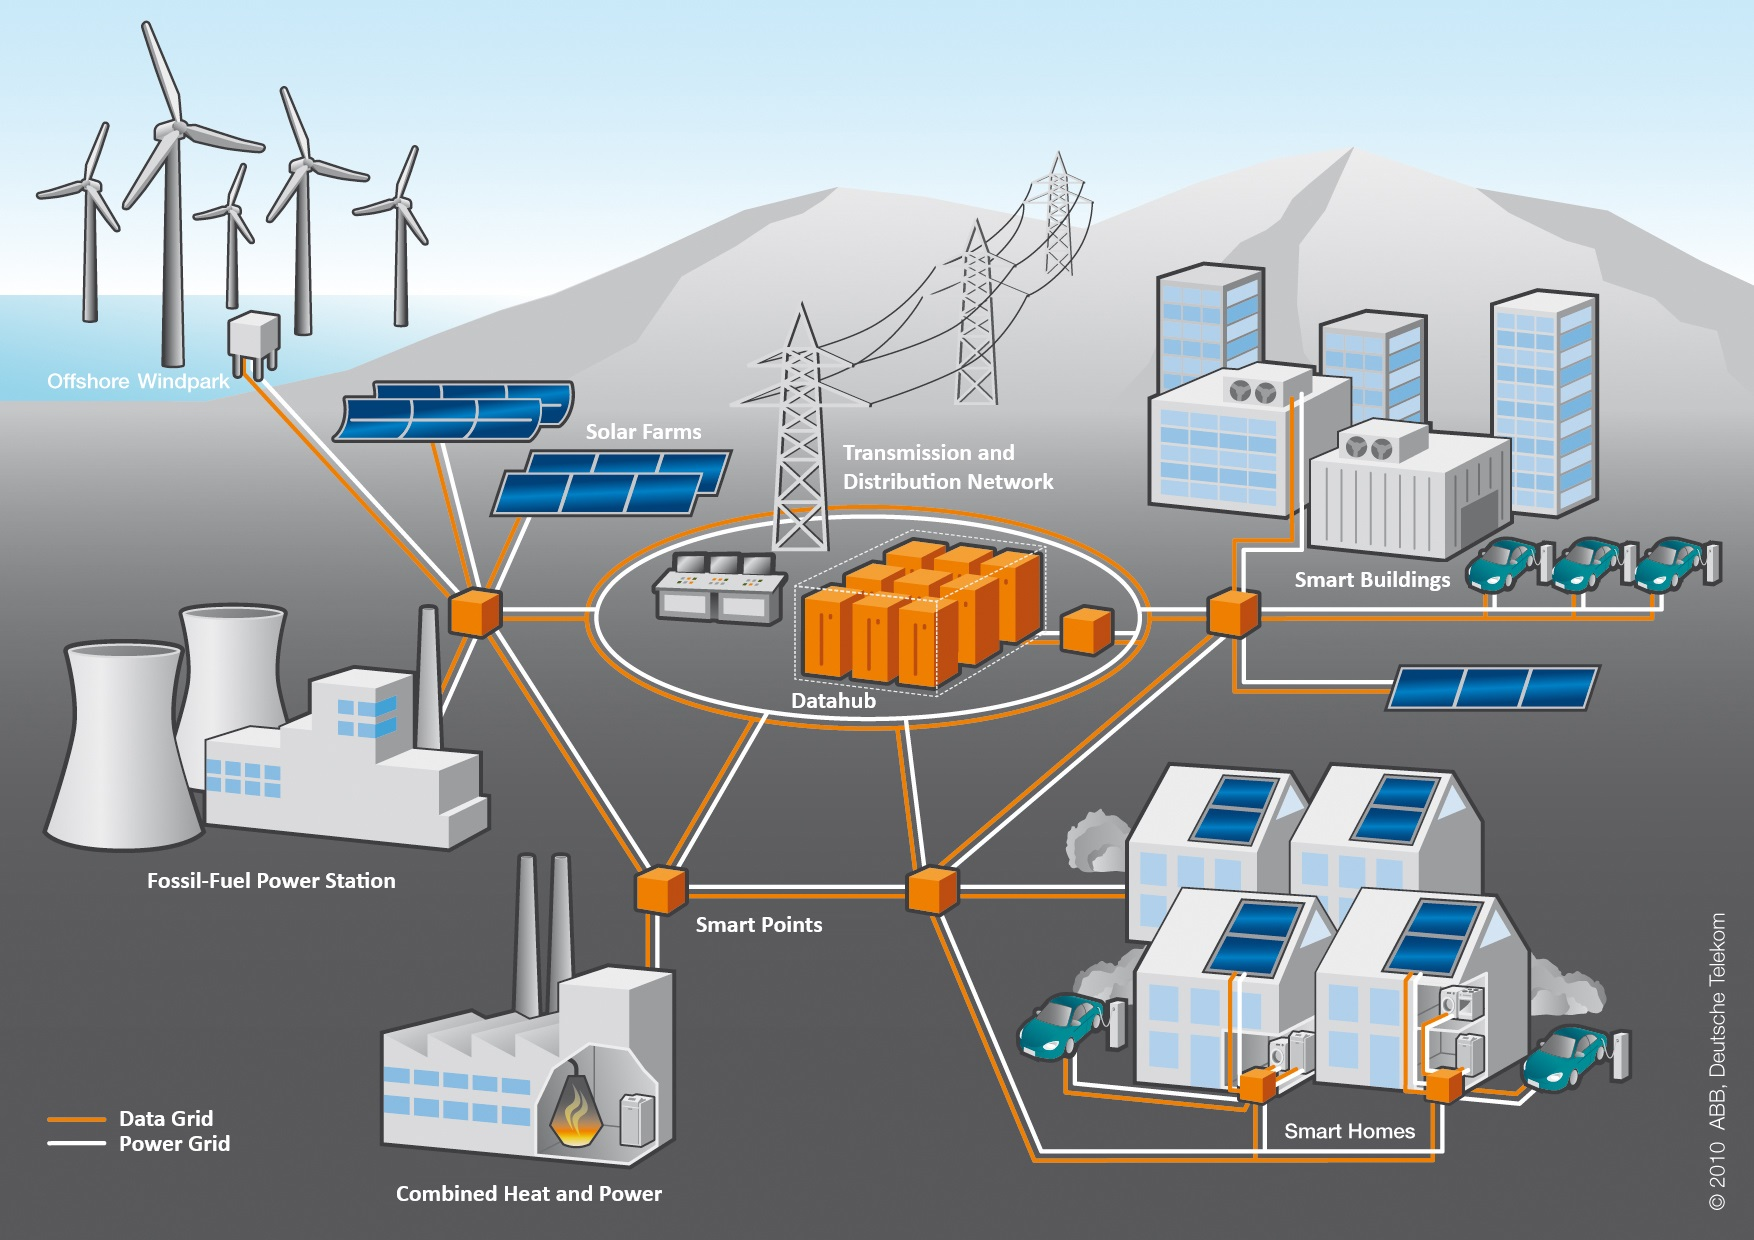
\includegraphics[width=\textwidth]{figures/SmartGrid_Ueberblick_ohneLegende.jpg}
	\caption{Smart grid outline.\\
		(Source: {\scriptsize\url{https://www.telekom.com/medien/bild-ton-und-infografiken/infografiken/155030}})}
	\label{fig:background:smartgrid}
\end{figure}

\subsection{Problems}
In regards to enabling an EU-wide smart grid, there are bound to be problems, as this is an immense project.
This roll-out will not be the same in every nation, as each nation has its own infrastructure and differs in which parts of their electrical grids are public and which are part of the free market.
However, some shared problems still exist, such as privacy, conflict of interest, and attack vulnerabilities \cite{offswitch} \cite{smart_meter_survey} \cite{security_economics}.

\subsubsection{Different architectures}
% Italy - regulated monopoly (supplier and distibutor is the same?)
% Germany - Free market for both distributor (people buy smart meter device/maintenance) and supplier
% UK - Centralized government-licensed monopoly
% DK - Centralized through 60 government-regulated distributors, datahub contains/controls all power usage data
\mikael{I am far from certain of the details here. What is important to mention?}

\subsubsection{Privacy}
With the adaptation of smart meters it will be viable to collect power usage data more often.
This is possible as it can be done remotely, whereas earlier a display would have to be read on the physical electrical meter.
It also makes sense to have more readings, as tariffs will vary more, and therefore more measurements are needed to match prices during tariff-determined periods.

This possibility of higher granularity meter readings can be exploited in several ways and by different actors.
The supplier would like this information in order to better tailor prices for a certain customer, thus limiting competition as their competitors do not possess this information.
If the power usage data was obtained by an electronics vendor, they could use it to target certain advertisements, based on what devices they detect (or don't) through the power usage.
Anyone with malicious intent could use the power data to determine who, if anyone, is home (e.g. burglars).
Finally, the government could use this data to surveil the public.

Some important issues with smart meters and their measurements are therefore:
\begin{itemize}
	\item Who owns the data?
	\item Who should be able to access the data?
	\item With what granularity should supplier/government/user be able to access the data?
	\item How do we ensure that only the correct people have access to the smart meter and its data?
\end{itemize}

\subsubsection{Conflict of interest}
The actors have different interests and potential gains with a smart grid.
Governments generally want lower consumption for environmental reasons.
They especially want consumption down during peak hours, in order to avoid the usage of environmentally unfriendly energy sources.
Depending on tariffs, suppliers might also want power consumption down during peak hours if they cannot provide enough, from their perspective, cheap energy.
However, suppliers generally want high consumption, so that they can sell more power and thus make more money.
Consumers want to use power as needed, but at lower costs (some consumers might also have environmental considerations).

These relations spark conflicts of interest:
\begin{itemize}
	\item Should governments be able to control user power consumption? If so, how?\footnote{E.g. carbon rationing in the UK \cite[]{security_economics}}
	\item Should others than the user be able to turn off the power \cite[]{offswitch}? If so,
	\begin{itemize}
		\item who should be able to use this?
		\item how should it work? (With abuse in mind.)
	\end{itemize}
	\item How, and by who, should smart appliances be managed?
\end{itemize}

\subsubsection{Vulnerabilities}
As it is now, people already tamper with the mechanical electrical meters.
Turning these mechanical meters into smart meters will not remove attacks, but will only open up for new attacks.
Switching to smart meters opens up for digital attacks, which include attacks that are general to any publicly exposed unit, or any unit that sends data over public networks.

Vulnerabilities will be further discussed and analysed in a threat analysis or whatever.